


\section{Moving Skarabs}


\textbf{WARNING}:\textit{ do not try to move the skarabs right after stopping or starting a subarray. The SKARABs need a couple of minutes to restart. Otherwise, they will not be found by the script, and will be left behind on the unwanted cmc.}\\

\subsection{CMC IP addresses}
The IP addresses for different machines are:
\begin{itemize}


	\item[] \server{cmc1: 10.103.254.1} and name: \server{cmc1.cbf.mkat.karoo.kat.ac.za}
\item[] \server{cmc2: 10.103.254.3} and name: \server{cmc2.cbf.mkat.karoo.kat.ac.za}, 

\item[] You can use the IP addresses or hostnames interchangeably (whichever you prefer) 


\item[] The cbf\_support repository is on git. You can clone it from:\\
git clone \url{https://github.com/ska-sa/cbf_support}
\end{itemize}
\subsection{Check the number of SKARABS}
In order to check the number if SKARABS are available in the CMC use the following
commands on the obs machine before attempting to move them. There should be about 220(as at 2020-01-06, but more will come) if they were all moved. If there are less, wait a couple
of minutes for them to restart.

\begin{lstlisting}[style=DOS]
kcpcmd -t 10 -s cmc1.cbf.mkat.karoo.kat.ac.za:7147 resource-list | grep "up$" | wc -l
\end{lstlisting}
(this will give you the number of skarabs available on cmc1.) 
\begin{lstlisting}[style=DOS]
kcpcmd -t 10 -s cmc2.cbf.mkat.karoo.kat.ac.za:7147 resource-list | grep "up$" | wc -l
\end{lstlisting}
(this will give you the number of skarabs available on cmc2.) \\

\subsection{Moving SKARABS}
If moving to cmc1 use -m cmc1:
\begin{lstlisting}[style=DOS]
./usersnfs/cbf_support/./cmc_manage_skarabs.py -m cmc1 -a 5 6 7 8 9 10 11 12 13 14 15 16 17 18 
 -k cmc1 cmc2
\end{lstlisting}
If moving to cmc2 use -m cmc2:
\begin{lstlisting}[style=DOS]
./usersnfs/cbf_support/./cmc_manage_skarabs.py -m cmc2 -a 5 6 7 8 9 10 11 12 13 14 15 16 17 18  -k cmc1 cmc2
\end{lstlisting}




This will connect to all the switches, discover which skarabs are currently online on the various ports, and move them to the requested master controller (-m switch).



\section{Global Synchronisation}

This script seeks to synchronize all digitisers to the Digitiser Master Controller so that signal/data coming into the correlator is in sync and correlates. 
\begin{itemize}
\item{} Ensure epoch sync on all usable digitisers (all bands) is done for the day
\item{} In the GUI, verify that all subarrays are inactive:
\begin{lstlisting}[style=DOS]
ssh kat@obs.mkat.karoo.kat.ac.za
run /home/kat/katsdpscripts/utility/global_sync.py
--observer= name --proposal-id=OPS-23

\end{lstlisting}



\item To check that all digitisers are synced and have the same epoch time, in the
same ipython session
\begin{lstlisting}[style=DOS]
ipython
import katuilib
configure()
kat.report_sensors('epoch','all')
\end{lstlisting}

\item Three ways to check time remaining for the next global sync
\begin{itemize}


\item [$\circ$] Check the Next Global Sync from the active subarray in the GUI (see \textbf{Figure}~\ref{fig:image115}). This gives
indication on what is the time remaining before the next global sync is
done.
\begin{figure}[H]
	\centering
	%\includegraphicsdpi{100}{}{bur1.png}     
	
\includegraphics[scale=0.46]{Chapters/images/image115.png}
	
	%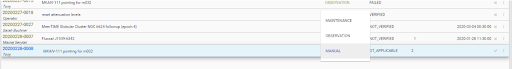
\includegraphics[resolution=100]{bur1.png}
	\caption{Global sync time remaining alert on the GUI }
	\label{fig:image115}
\end{figure}
\item [$\circ$] From the sensor list by typing \sensor{remaining} as shown in \textbf{Figure}~\ref{fig:image121}.
\begin{figure}[H]
	\centering
	%\includegraphicsdpi{100}{}{bur1.png}     
	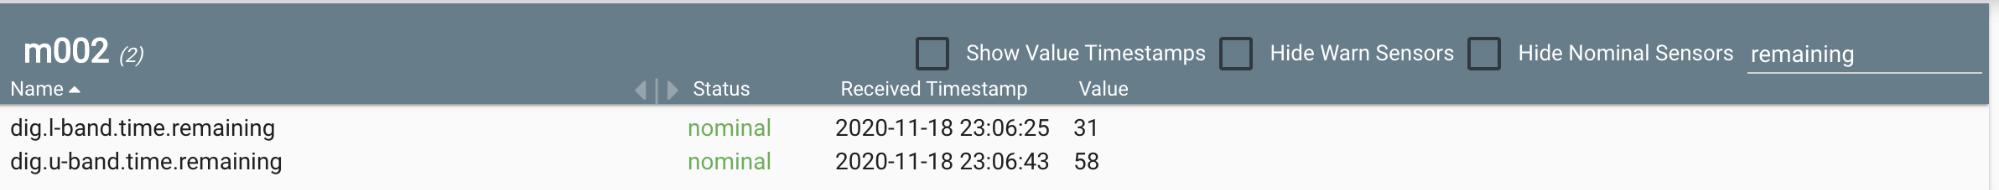
\includegraphics[scale=0.23]{Chapters/images/image121.png}
	
	%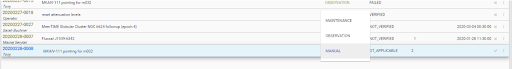
\includegraphics[resolution=100]{bur1.png}
	\caption{Global sync time remaining alert in sensor list}
	\label{fig:image121}
\end{figure}
\item [$\circ$] On IRC there is a reminder that reminds when to run a Global sync counting down
hourly from 15 hours left .
\end{itemize}
\end{itemize}


\section{Setting up digitisers}
\subsection{ Configured Ipython Session}
\begin{lstlisting}[style=DOS]
ssh kat@obs.mkat.karoo.kat.ac.za
ipython
import katuilib
configure_cam('camcam', 'all')
\end{lstlisting}

\subsection{ Mark Digitiser Absent}
The digitiser will be marked absent if there is maintenance work on the AP which
may cause the power to be switched off to the digitiser. It is also recommended that it
is marked absent if the AP will be out for maintenance for a long time.
In a configured ipython session run the following commands:
\begin{lstlisting}[style=DOS]
cam.m0xx.req.dig_select_band('0')
cam.m0xx.req.digitiser_absent('l', timeout=60)
\end{lstlisting}

In this case ‘l’ represents L-band digitiser
\subsection{Mark digitiser ready}
When the digitiser was marked absent or the new digitiser was installed in the AP, it
is required that it must be set ready for operations. Still in a configured ipython
session run the following commands:
\begin{lstlisting}[style=DOS]
cam.m0xx.sensor.dig_selected_band.get_value()
cam.m0xx.req.digitiser_ready('l', timeout=60)
cam.m0xx.req.dig_select_band('l', timeout=60)
\end{lstlisting}

If all digitisers were marked absent previously, this command above must be run for
all different bands, i.e. 'l' must be replaced with ‘u’ for UHF band digitiser. There is
no need to set an S-band digitiser at this stage.
\section{ Requesting which receptors have UHF$-$band digitisers}
In order to determine which antennas have UHF band digitisers installed on them, you will
run the following commands:
On the machine: ssh kat@obs.mkat.karoo.kat.ac.za and run the following commands.
\begin{lstlisting}[style=DOS]
u=`kcpcmd -t 60 -s 10.103.254.2:7147 list-digitisers | grep "u as
ready" | cut -d ' ' -f 2` && echo $u
\end{lstlisting}
If you prefer a list format do the following:
\begin{lstlisting}[style=DOS]
u=`kcpcmd -t 60 -s 10.103.254.2:7147 list-digitisers | grep "u as
ready" | cut -d ' ' -f 2` && echo -e "\n$u\n"
\end{lstlisting}


\section{ Digitiser Health}
In order to see the status of each digitiser that is operational one can use the following
commands to check for errors and health of each digitiser.
For L-band:
\begin{lstlisting}[style=DOS]
kat@obs.mkat.karoo.kat.ac.za:~$ dig-stats
\end{lstlisting}
For U-band:
\begin{lstlisting}[style=DOS]
kat@obs.mkat.karoo.kat.ac.za:~$ dig-stats 10.103.254.2:7147 u
\end{lstlisting}

\section{ Power sensors}
Important digitiser sensors to note for operations are power level The digitiser receives RF
signals from the receiver and the levels are measured at the inputs of the digitiser by the
RFCU. From the CAM GUI sensor list, filter for rfcu i.e. rfcu.*.power.  \textbf{Figure}~\ref{fig:image83} shows the power levels for each polarisation of m006.
\begin{figure}[H]
	\centering
	%\includegraphicsdpi{100}{}{bur1.png}     
	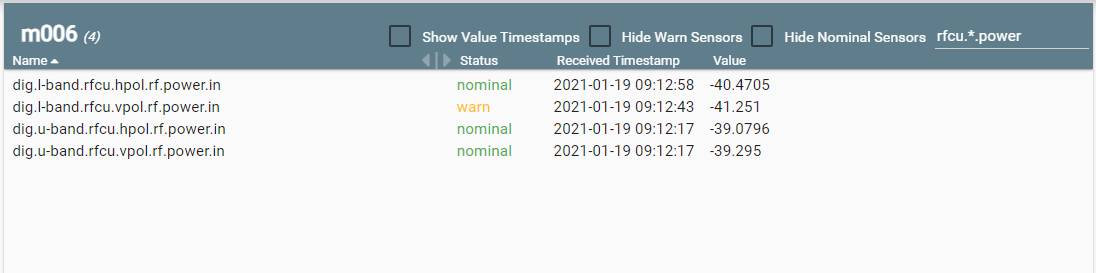
\includegraphics[scale=0.39]{Chapters/images/image83.png}
	
	%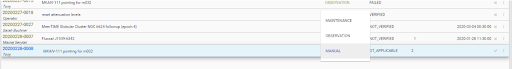
\includegraphics[resolution=100]{bur1.png}
	\caption{Global sync time remaining alert in sensor list}
	\label{fig:image83}
\end{figure}
The power levels for inputs on the L-band should be between -42dBm and -45dBm (when
not observing) and if they exceed these values this will be shown as warning. Low power
may mean that the LNA on the receiver are switched OFF or high power might mean AP is
pointing at a strong source or ground.\\

The second power level sensors for the digitisers are the ADC power levels which are
measured at the input of the ADC after the gains have been applied. The gains depends on
the attenuation levels which can be manually set, but we use separate scripts in setting and
refining attenuations. This is important to configure the attenuations so that all antennas
have the same output power levels. From the CAM GUI sensor list, filter for adc power i.e.
adc.*.power.in. \textbf{Figure}~\ref{fig:image51} shows the power levels for each polarisation of m006.
\begin{figure}[H]
	\centering
	%\includegraphicsdpi{100}{}{bur1.png}     
	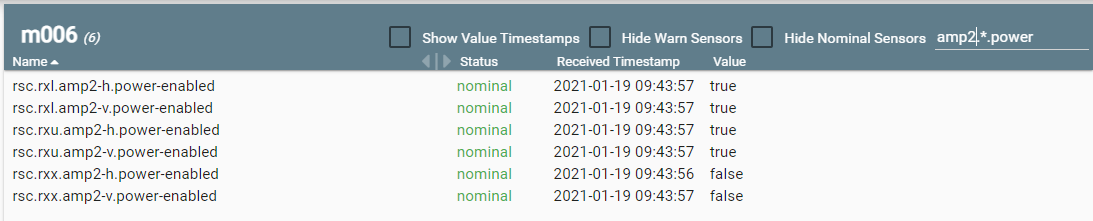
\includegraphics[scale=0.4]{Chapters/images/image51.png}
	
	%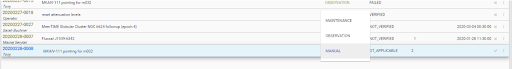
\includegraphics[resolution=100]{bur1.png}
	\caption{Global sync time remaining alert in sensor list}
	\label{fig:image51}
\end{figure}
It is recommended that the refine attenuations script should be run after building a new
subarray and the set attenuations script be run if there is a change in the signal chain i.e. a
Receiver or a Digitiser was replaced.
\section{ Updating config for a replaced digitiser}
Digitisers normally have their config files updated before they are handed over to
Operations. If a digitiser is replaced, it's serial number needs to be updated in CAM's
katconfig configuration files. This will require someone from the operations team to perform
github updates. The procedure to do that is shown below.\\

Note: Swaps done in S-band does not need updates in katconfig, because S-band
packetisers don’t use serial numbers, but instead use IP addresses according to the receptor number which gets set in the packetiser itself during installation.  This is their way
of communicating with MeerKAT. Hence the IP address never has to change when S-band
packetisers are replaced.
There are two different procedures which you can choose to follow:
\subsection{ On the terminal}
\begin{lstlisting}[style=DOS]
ssh kat@ops.kat.ac.za
cd katconfig/static/antennas/
git checkout master
git pull
git checkout karoo
git pull
git checkout -b update_m0XX_dig_config
\end{lstlisting}

If the response is:
\begin{lstlisting}[style=DOS]
fatal: A branch  named update\_m0XX\_dig_config already exists.
\end{lstlisting}
then rerun the command, but exclude “-b” this time.
\begin{lstlisting}[style=DOS]
git branch
\end{lstlisting}
 This should give: \option{*update\_m0XX\_dig\_config} 
\begin{lstlisting}[style=DOS]
ls
vi m0XX.conf 
\end{lstlisting}
(you can also use \option{nano m0XX.conf} whichever you comfortable with)

Type the letter “i” in order to edit the file.
The file format should be for example:
\begin{lstlisting}[style=DOS]
digitiser_l = ready:dig-041
\end{lstlisting} 
(we want to change this to the new serial number, i.e 064 for
example, to have \option{digitiser\_l = ready:dig-064})


any digitisers not installed should be of the format: 
\begin{lstlisting}[style=DOS]
digitiser_x = absent
\end{lstlisting}
Save the file and exit (press Esc, then type ":wq!")

\begin{lstlisting}[style=DOS]
git diff (shows changes you have made, check they are correct)
git add .
git commit -m "Updating (relevant band) digitiser serial no to 0XX on
m0XX"
git push --set-upstream origin update_m0XX_dig_config
\end{lstlisting}
\subsection{ On Github website}
\begin{itemize}


\item  Go to github:  \url{https://github.com/ska-sa/katconfig}
\item  Go to the new branch by clicking  on the dropdown list on available branches as shown in \textbf{Figure}~\ref{fig:image83} 
(should currently be on the karoo branch) and then selecting the branch name
of the new branch created .
\begin{figure}[H]
	\centering
	%\includegraphicsdpi{100}{}{bur1.png}     
	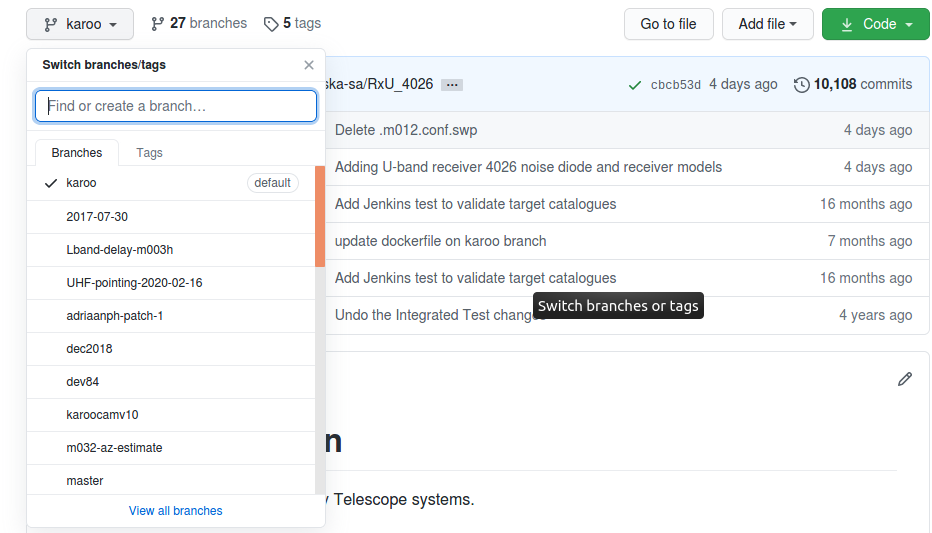
\includegraphics[scale=0.43]{Chapters/images/image108.png}
	
	%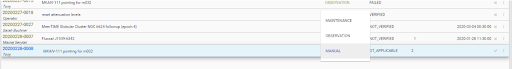
\includegraphics[resolution=100]{bur1.png}
	\caption{Github new branch select}
	\label{fig:image108}
\end{figure}

\item Create pull request from \option{update\_m0XX\_dig\_config} (name of branch created)
to karoo by clicking on “Pull request” at the top right as shown in \textbf{Figure}~\ref{fig:image73}.
\begin{figure}[H]
	\centering
	%\includegraphicsdpi{100}{}{bur1.png}     
	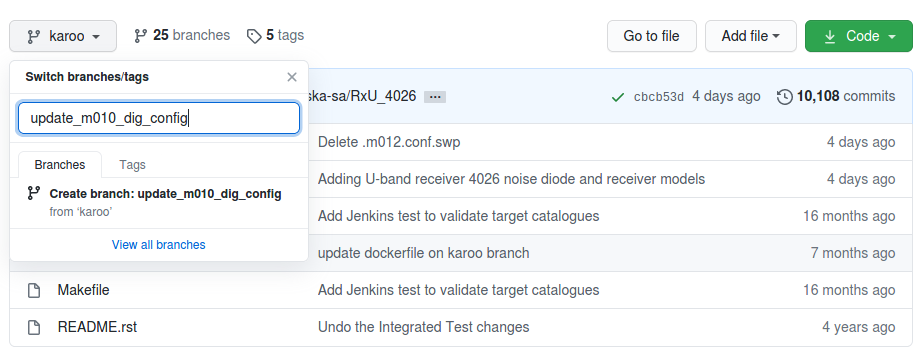
\includegraphics[scale=0.43]{Chapters/images/image73.png}
	
	%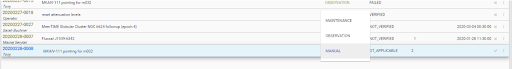
\includegraphics[resolution=100]{bur1.png}
	\caption{Github create pull request }
	\label{fig:image73}
\end{figure}



\item Make sure \option{base:karoo} and \option{compare:update\_m0XX\_dig\_config} is
selected. (Also make sure it’s only the files you have modified which are part
of the pull request - if you did the above steps properly that will be the case).
\item Then write a comment stating what you are doing, why (give Jira number if
applicable) and make the request out to Pieter Kotze. See an example in \textbf{Figure}~\ref{fig:image47}.
\begin{figure}[H]
	\centering
	%\includegraphicsdpi{100}{}{bur1.png}     
	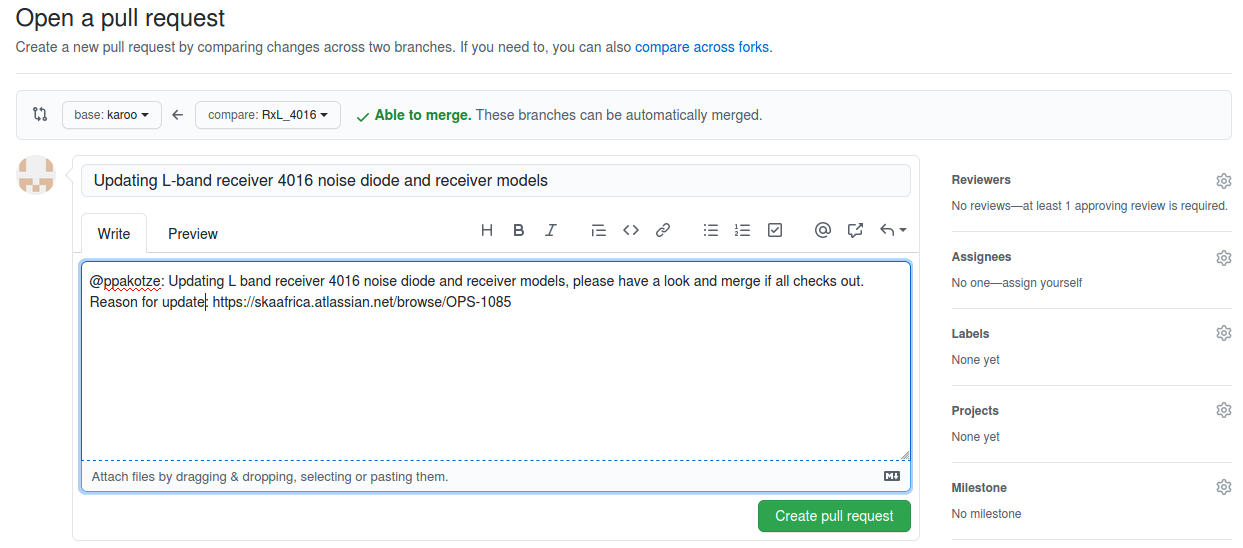
\includegraphics[scale=0.33]{Chapters/images/image47.png}
	
	%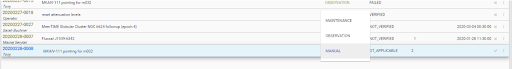
\includegraphics[resolution=100]{bur1.png}
	\caption{Github open pull request }
	\label{fig:image47}
\end{figure}
\item At the right hand side at the top next to “Reviewers”, click on the gear icon. It
will drop down a list of reviewers to choose from. Type “ppakotze” (see \textbf{Figure}~\ref{fig:reviewers}) in the
search field to find Pieter K and then click on Pieter K to request him to
approve your pull request (It will show a check mark next to his name, and
then under “Reviewers” you will see a yellow dot next to his name).

\begin{figure}[H]
	\centering
	%\includegraphicsdpi{100}{}{bur1.png}     
	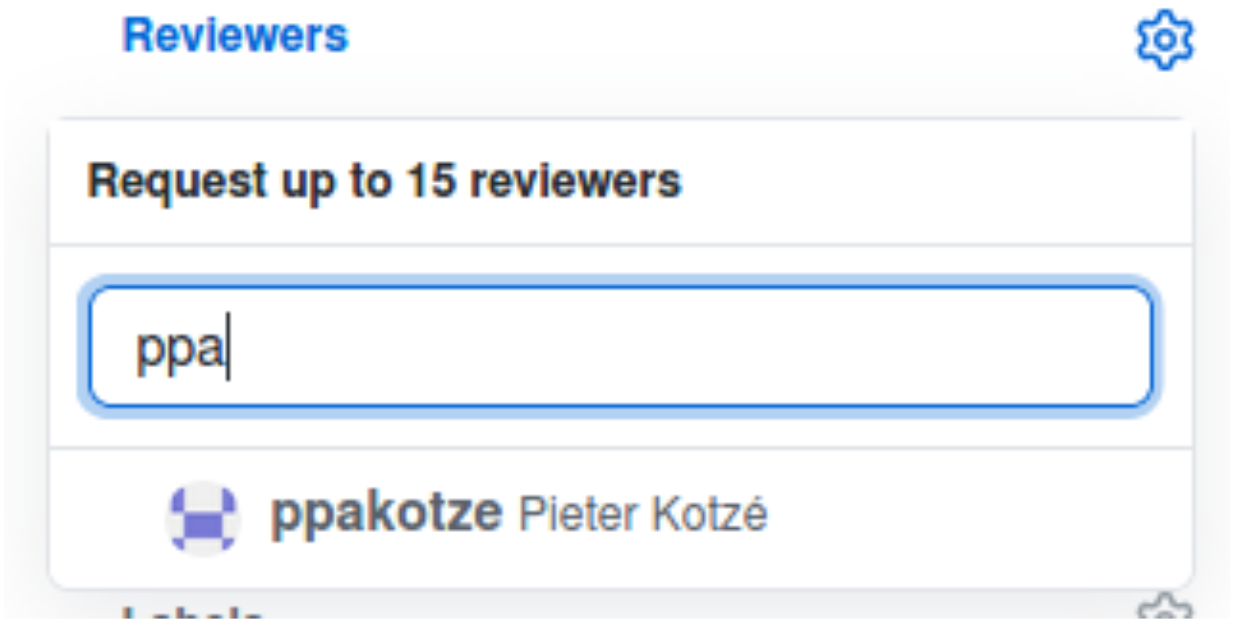
\includegraphics[scale=0.26]{Chapters/images/reviewers.png}
	
	%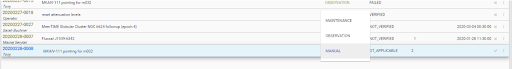
\includegraphics[resolution=100]{bur1.png}
	\caption{Github revievers dialogue }
	\label{fig:reviewers}
\end{figure}
\item Then click on “Create pull request”.\\
\textit{ Note: After Pieter K approves the pull request, he usually also merges
the pull request, but sometimes you have to do the merging yourself.
You do this by going to the pull request after it has been approved,
and then click on “Merge pull request” at the bottom and then “Confirm
merge”}
\end{itemize}






	